\section{Parallel MOEAs for the VNFPP}
\label{sec:algorithms}

In this section we outline the algorithms evaluated in this work and the genetic operators used to solve the VNFPP. First we describe the PMOEAs we evaluated and then we describe the genetic operators we have constructed to solve the VNFPP. 

\subsection{Parallel MOEA Frameworks}
PMOEAs can be grouped into three categories: master/slave algorithms, multiple-deme and isolated-deme algorithms \cite{Cantu-PazG99}. Each parallel algorithm distributes tasks over $N_T$ threads. In this work we evaluated a PMOEA from each category against a serial MOEA that does not use multithreading. The remainder of this section describes these algorithms in detail.

A serial MOEA is an evolutionary algorithm that only uses a single process. For this category, we selected the well known NSGA-II \cite{DebAPM00} algorithm, illustrated in Fig. \ref{fig:nsgaii}. NSGA-II maintains a population of $N$ parent solutions. A population of $N$ child solutions are generated via mutation and crossover of the parent population. Both populations are combined and then fast nondominated sorting and crowding distance procedures are used to determine which solutions survive to become the parent solutions of the next generation. This process repeats until the stopping condition is met. NSGA-II has been shown to be effective on a range of multiobjective optimization problems previously, including the VNFPP \cite{BillingsleyLMMG20}. Additionally, several parallel variants of NSGA-II exist, allowing for a fair comparison between single and multithreaded algorithms.

A master/slave algorithm has a single `master' thread that allocates tasks to `slave' threads. Once the slave threads are finished, the master thread aggregates the results. In this work we parallelise NSGA-II using this architecture, hereafter referred to as MS-NSGA-II (illustrated in Fig. \ref{fig:msnsgaii}). In this implementation each thread performs crossover, mutation and evaluation to produce $N / N_T$ solutions. Afterwards the solutions from each thread are aggregated to form the child population. As in NSGA-II, fast nondominated sorting and crowding distance procedures are used to select the parent population for the next generation. This process repeats until the stopping condition is met.

\begin{figure*}[t]
    \begin{minipage}{\textwidth}
        \centering
        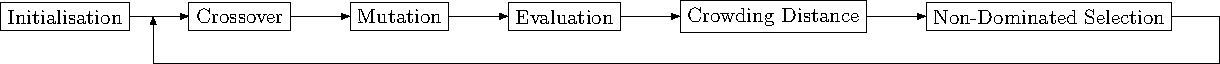
\includegraphics[width=\textwidth]{figures/algorithms/nsgaii}
        \subcaption{NSGA-II \cite{DebAPM00}}
        \label{fig:nsgaii}
    \end{minipage}
    \vspace{2.5em}

    \begin{minipage}{\textwidth}
        \centering
        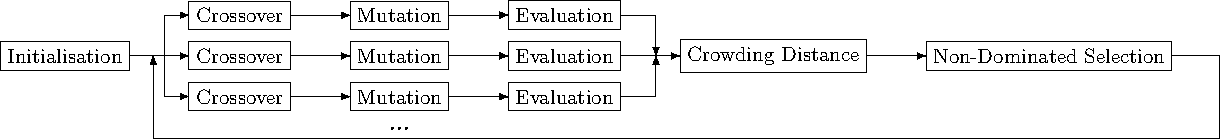
\includegraphics[width=\textwidth]{figures/algorithms/msnsgaii}
        \subcaption{MS-NSGA-II}
        \label{fig:msnsgaii}
    \end{minipage}
    \vspace{2.5em}

    \begin{minipage}{\textwidth}
        \centering
        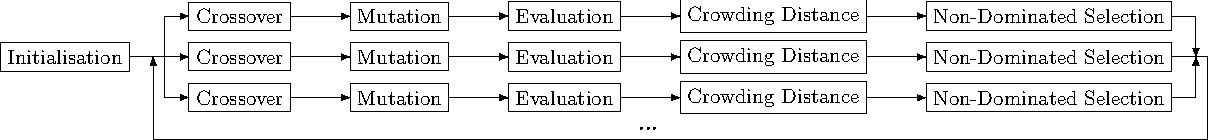
\includegraphics[width=\textwidth]{figures/algorithms/mdnsgaii}
        \subcaption{MD-NSGA-II \cite{RobergeTL13}}
        \label{fig:mdnsgaii}
    \end{minipage}
    \vspace{2.5em}

    \begin{minipage}{\textwidth}
        \centering
        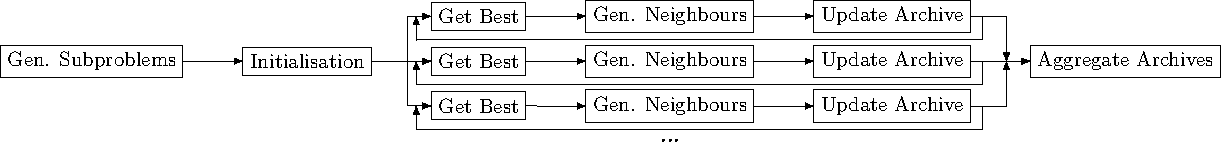
\includegraphics[width=\textwidth]{figures/algorithms/ppls}
        \subcaption{PPLS/D \cite{ShiZS20}}
        \label{fig:pplsd}
    \end{minipage}

    \vspace{1em}
    \caption{The four MOEAs we considered in this work. NSGA-II is a serial algorithm whilst the remaining parallelize some or all steps.}
    \label{fig:algorithms}
\end{figure*}

A multiple-deme algorithm evolves multiple subpopulations in parallel and periodically exchanges solutions between them. In this work we use the algorithm proposed by Roberge et al. \cite{RobergeTL13}, hereafter referred to as MD-NSGA-II, which uses a multiple-deme architecture (illustrated in Fig. \ref{fig:mdnsgaii}). Roberge et al. first produce a set of initial solutions and group them into $N_T$ equal sized subpopulations. The variation, evaluation and selection operators from NSGA-II are performed on each subpopulation in parallel. After a set number of generations, the subpopulations are aggregated into a new population and then randomly redistributed back into $N_T$ subpopulations. This process repeats until the stopping condition is met.

An isolated-deme algorithm also evolves multiple subpopulations but does not exchange information between the subpopulations. In this work we use the isolated-deme algorithm PPLS/D \cite{ShiZS20} (illustrated in Fig. \ref{fig:pplsd}). PPLS/D first decomposes the objective space into $N_T$ scalar objective optimization subproblems. The algorithm maintains a population of unexplored solutions and an archive of non-dominated solutions for each subproblem. First, a solution is added to the unexplored population of each subproblem. Next, for each subproblem the algorithm selects the best solution from the unexplored population and generates a set of neighboring solutions. A neighboring solution is added to the unexplored population and the non-dominated archive if it is: 1) closer to the subproblem that generated it than any other subproblem, as measured by the angle between the solution and the subproblems and 2) is either a better solution to the subproblem than the current best solution or if it is not dominated by any solutions in the non-dominated set of the subproblem. Once the stopping condition is met, the algorithm aggregates the non-dominated archives from each subproblem and returns the overall non-dominated solutions.

PPLS/D was designed for unconstrained optimization problems, so required modification to fit the VNFPP. In our variant, an infeasible solution is accepted into the unexplored population only if there are no more feasible solutions in the population. 

Additionally, to determine how PPLS/D is affected by the number of subproblems used, we generate $N$ subproblems that are placed into $N_T$ equally sized groups. Each subproblem in a group is executed in series and each group is executed in parallel. This technique produces solutions with the same solution quality as if greater numbers of threads were available whilst not unfairly benefitting PPLS/D.

\subsection{Genetic Operators}

\begin{figure}[t]
    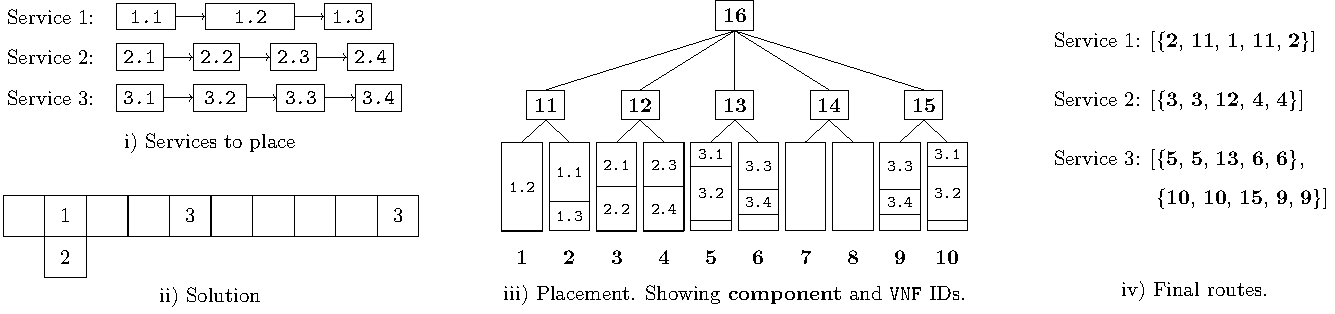
\includegraphics[width=\textwidth]{figures/algorithms/mapping}
    \caption{A partial mapping from genotype to phenotype showing the assignment of services to servers.}
    \label{fig:mapping}
\end{figure}

As this work focusses on the benefits of parallelisation, we use existing genetic operators that were designed for the VNFPP. In particular we use operators we demonstrated to be effective in earlier work \cite{BillingsleyLMMG20}. These operators use a genotype-phenotype representation where genetic operators consider a simplified solution representation (the genotype) which is converted into the `true' solution representation (the phenotype) to be evaluated. In our implementation, the genotype is an array of vectors where each vector represents a server in the datacenter (see Fig. \ref{fig:mapping} ii). Each vector contains zero or more service instances. The phenotype is the set of paths for each service (see Fig. \ref{fig:mapping} iv). The genotype-phenotype mapping has two parts: expansion and routing as shown in Fig. \ref{fig:mapping}. The expansion step iterates over each server in the genotype. When a service instance is encountered, the algorithm places each VNF of the service on the closest server that can accommodate it. The routing step finds the set of shortest paths between each VNF and combines them to form a path.

MD-NSGA-II and MS-NSGA-II require initialization, mutation, crossover and evaluation operators. PPLS/D additionally requires a local search operator. Since all services are considered equally important, the initialization operator always generates genotypes where each service has the same number of service instances. The operator first determines the maximum number of service instances that can be placed in a datacenter whilst meeting this constraint. Then it generates a range of solutions between the maximum and minimum number of service instances that can be placed. The mutation operator has an equal probability of 1) swapping the contents of two servers, 2) adding a random service instance to a random server and 3) removing a random service instance from a server. The same operator is used to generate neighbors in PPLS/D. Crossover is performed using the N-Point crossover.